\documentclass[11pt]{article}
\usepackage[utf8]{inputenc}
\usepackage[T1]{fontenc}
\usepackage{fixltx2e}
\usepackage{graphicx}
\usepackage{longtable}
\usepackage{float}
\usepackage{wrapfig}
\usepackage{rotating}
\usepackage[normalem]{ulem}
\usepackage{amsmath}
\usepackage{textcomp}
\usepackage{marvosym}
\usepackage{wasysym}
\usepackage{amssymb}
\usepackage{capt-of}
\usepackage{hyperref}
\tolerance=1000
\usepackage{minted}
\usepackage{color}
\usepackage{listings}
\usepackage{grffile}
\usepackage[inline]{enumitem}
\usepackage{setspace}
\usepackage{tikz}
\usepackage{subcaption}
\usepackage{xcolor}
\usepackage{fancyvrb}
\hypersetup{
colorlinks,
linkcolor={red!50!black},
citecolor={blue!50!black},
urlcolor={blue!80!black}
}
\usepackage{setspace}%% The linestretch
\singlespacing
\usepackage[format=hang,indention=0cm,singlelinecheck=true,justification=raggedright,labelfont={normalsize,bf},textfont={normalsize}]{caption} %
\usepackage{vmargin}
\setpapersize{A4}
\setmarginsrb{2.5cm}{1cm}% links, oben
{2.5cm}{2cm}% rechts, unten
{12pt}{30pt}% Kopf: Höhe, Abstand
{12pt}{30pt}% Fuß: Höhe, AB
\usepackage{upquote}
%  use straight quotes when printing a command in minted
\AtBeginDocument{%
\def\PYZsq{\textquotesingle}%
}
\definecolor{mintedbackground}{rgb}{0.95,0.95,0.95}
\setlength{\parindent}{0pt}
\setlength{\parskip}{\baselineskip}
\definecolor{mintedbackground}{rgb}{0.95,0.95,0.95}
\definecolor{mintedBg}{rgb}{0.95, 0.95, 0.95}
\definecolor{blockBg}{rgb}{0.6, 0.6, 0.95}

%% define styles for different codes
\newminted{cpp}{linenos, bgcolor=blockBg, fontsize=\footnotesize}
%% then use \begin{cppcode}
\newminted{c}{linenos, bgcolor=mintedBg, fontsize=\footnotesize}
\newminted{perl}{linenos, bgcolor=mintedBg, fontsize=\footnotesize}
\newminted{r}{linenos, bgcolor=mintedBg, fontsize=\footnotesize}


%% I detest indentation in footnotes etc, so try this:
\makeatletter
\renewcommand\@makefntext[1]{\noindent\makebox[0em][r]{\@makefnmark}\footnotesize#1}
\makeatother
%% the makeatletter and makeatother are required to allow me to
%% to change the macro beginning with an @. (though when I call it
%% I don't use the @ ... 

%% this should handle non-breaking space
%% characters.
\DeclareUnicodeCharacter{00A0}{~}

\renewcommand\scriptsize\normalsize

\author{Martin Jakt\thanks{University of Nordland, Norway}}
\date{\textbf{Bioinformatics \& Genomics}}
\title{\textbf{Looking at Big Data} (2015-10-15)}
\hypersetup{
 pdfkeywords={},
  pdfsubject={},
  pdfcreator={}}
\begin{document}

\maketitle
%\tableofcontents

\section{Playing with data}
\label{sec-1}
In this practical class we will learn how to take a reasonably
big pile of numbers, look at it and get some idea of how the
data is structured. The data we will use is expression data from
rat using Affymetrix oligonucleotide arrays. Affymetrix arrays contain
a 2 dimensional array of oligonucleotide sequences which are manufactured
by light directed chemical extension of the oligonucleotides on the
array itself. This differs from the typical array where an oligonucleotide
solution is spotted, and offers a higher density of features; it's
an approach directly inspired by and analogous to the way in which
computer chips are fabricated by photolithography.

On Affymetrix chips each transcript is represented by a set of 25 base
long oligonucleotides (usually 22) of which half are perfectly 
complementary to the transcript sequences they represent and half contain
a single, central mismatch. The signals from each set of oligos
are combined to give a single estimate of expression level. The data which
we will look at contains only the final estimates of expression levels and
does not include the lower level individual probe level data. The individual
probe data provides additional information that can be used to assess both
the integrity of samples and transcript level estimates. However, that
is very specific to the Affymetrix platform and as such is not really
suitable for a general introduction to looking at numbers.

\subsection{Getting the data into R}
\label{sec-1-1}
The data we will look at today can be obtained from the
Gene Expreession Omnibus (GEO) database hosted at the
NCBI (National Center for BioInformatics):

\url{http://www.ncbi.nlm.nih.gov/geo}

by searching for GDS3850 and following the link pointing at:\\
GDS3850\_full.soft\\

Alternatively you can download the file from fronter in the obvious place.

The GDS3850\_full.soft file contains both descriptions of the samples
the expression data itself and information about the genes that are
represented by the probes on the array. The formal specification of the
file format can be found at:\\
\url{http://www.ncbi.nlm.nih.gov/geo/info/soft.html#format}

In theory one can use the file format specification and write some code
to extract the relevant information. In practice, you pretty much always
have to look at the sample descriptions within in order to understand
the structure of the experimental data. This is partly because it is
not easy to formalise the description of experimental samples, but also
because everyone seems to submit their data in a different way. Unfortunately
there are not many good shortcuts.

%% fancyvrb use Verbatim rather than verbatim?
\begin{figure}[ht]
\begin{Verbatim}[fontsize=\small]
^DATABASE = Geo
!Database_name = Gene Expression Omnibus (GEO)
!Database_institute = NCBI NLM NIH
!Database_web_link = http://www.ncbi.nlm.nih.gov/geo
!Database_email = geo@ncbi.nlm.nih.gov
!Database_ref = Nucleic Acids Res. 2005 Jan 1;33 Database Issue:D562-6
^DATASET = GDS3850
!dataset_title = Peroxisome proliferator-activated receptor-$\gamma$ ligand treatment: adipose tissue, skeletal muscle, and liver
!dataset_description = Analysis of 3 tissue types from lean and insulin resistant, obese Zucker rats untreated or treated with 1 of 4 PPAR$\gamma$ ligands (pioglitazone, rosiglitazone, troglitazone, AG035029).  Results provide insight into the role of PPAR$\gamma$ as an essential mediator for maintenance of body insulin sensitivity.
!dataset_type = Expression profiling by array
!dataset_pubmed_id = 20959535
!dataset_platform = GPL341
...
...
!subset_description = lean (fa/+)
!subset_sample_id = GSM533029,GSM533030,GSM533031,GSM533011,GSM533012,GSM533013,GSM532993,GSM532994,GSM532995
!subset_type = genotype/variation
^SUBSET = GDS3850_2
!subset_dataset_id = GDS3850
!subset_description = fatty (fa/fa)
!subset_sample_id = GSM533038,GSM533039,GSM533040,GSM533035,GSM533036,GSM533037,GSM533032,GSM533033,GSM533034,GSM533023,GSM533024,GSM533025,GSM533026,GSM533027,GSM533028,GSM533020,GSM533021,GSM533022,GSM533017,GSM533018,GSM533019,GSM533014,GSM533015,GSM533016,GSM533005,GSM533006,GSM533007,GSM533008,GSM533009,GSM533010,GSM533002,GSM533003,GSM533004,GSM532999,GSM533000,GSM533001,GSM532996,GSM532997,GSM532998,GSM532987,GSM532988,GSM532989,GSM532990,GSM532991,GSM532992
!subset_type = genotype/variation
^SUBSET = GDS3850_3
!subset_dataset_id = GDS3850
!subset_description = adipose tissue (epididymal)
!subset_sample_id = GSM532987,GSM532988,GSM532989,GSM532990,GSM532991,GSM532992,GSM532993,GSM532994,GSM532995,GSM532996,GSM532997,GSM532998,GSM532999,GSM533000,GSM533001,GSM533002,GSM533003,GSM533004
...
...  
\end{Verbatim}
\caption{Parts of the experiment and sample description part of GDS3850\_full.soft}
\label{soft1}
\end{figure}

Fig. \ref{soft1} shows part of the first section of the soft file. It contains a number of records
delineated by lines; these can be somewhat long and hence they overflow in the figure. If you
are using a Mac or Linux system you can look at this file using the \texttt{more} or \texttt{less}
programs from the terminal (eg. \texttt{more GDS3850\_full.soft}). There's probably
nothing very convenient on Windows (Wordpad might be ok, but as the file is a bit big you
may run into trouble. Notepad, doesn't work as it only recognises DOS style line ends.) 

The second part of the file contains the actual expression data and descriptions of the individual
features. This has very long lines, so I'm not even going to try to make a figure
out of it. Normally to extract the information from a file like this, I would write
a small Perl script and pick out the interesting bits (or possibly a bit of R depending
on the situation). However, not surprisingly, there is now an R-package avaiable from
Bioconductor that can be used to get most of the data from the soft file: \texttt{GEOquery}.
This can be used either to load data directly from NCBI, or from downloaded files.

\begin{listing}
\begin{rcode}
source("http://www.bioconductor.org/biocLite.R")

## the source command reads in R code from a file; usually the file
## contains function definitions that can then be in local scripts.

biocLite("GEOquery")
## this installs the GEOquery package and any packages that it
## depends on.

## to use the functions in the package you have to load it into
## your current session:

library(GEOquery)
\end{rcode}
\caption{Installing and loading the GEOquery package.}
\label{lis1}
\end{listing}

If you have downloaded the file to your local directory then you can
load the data into an object called \texttt{gds} by:

\begin{rcode}
  gds <- getGEO(filename="GDS3850_full.soft")
\end{rcode}

remembering of-course to make sure to provide a path to the file if
it is not present in the same directory as your R-session.
Alternatively you can try to load it directly from GEO by:

\begin{rcode}
  gds <- getGEO("GDS3850", destdir=".")
\end{rcode}
This will download the file, save a copy in your current directory
and load the data into the \texttt{gds} object. Note, that I haven't
tried doing this myself, and there is always a possibility that something
might end up somewhat not right.

\subsection{A first look at the data}
\label{sec-1-2}
\subsubsection{The metadata}
\label{sec-1-2-1}
The metadata (data that describes the experiment) can be obtained from the
\texttt{gds} object by the \texttt{Meta()} function.\footnote{I suspect that
the object returned by the getGEO function is what's known as an S4 class.
If so, then we should probably refer to \texttt{Meta()} as a slot or a method
rather than a function.} This will returned a named list. In R there is
an important distinction between vectors and lists. A vector is an ordered
collection whose elements can be accessed by their position or index. All
the elements of a vector have to be of the same type (eg., numeric, logical,
or character). A list is a special kind of vector that can contain
elements of different types (these can be anything, including lists and matrices).
Both vectors and lists can be named; that is individual elements of the vector
or list can also be accessed using a character based name. This can be done
either using the normal subsetting operators\footnote{For a vector these are
single square brackets, but for list elements double square brackets are required
for the actual element.} (eg. \texttt{listName[['elementName']]}) or
using the \texttt{\$} operator (\texttt{listName\$elementName}).

\begin{listing}
\begin{rcode}
  ## to print all the annotation to the screen:
  Meta(gds)
  ## to store it as a local variable
  gds.meta <- Meta(gds)
  
  ## to see the names of the list:
  names(gds.meta)

  ## to access a specific name:
  gds.meta$sample_id
  gds.meta$description

  ## we can also access these by
  gds.met[['sample_id']]
  gds.met['sample_id']
  ## these two return slightly different results. See if you
  ## can work out what (try using is.list() on the result).

  ## in fact you don't need to assign the result of Meta()
  ## to an object you can access things directly by:

  Meta(gds)$sample_id
  Meta(gds)$description
\end{rcode}
\caption{A first look at the metadata}
\label{lis2}
\end{listing}

Have a look at what the \texttt{Meta} function returns and see if you can
work out how the experiment was designed.

When I had a look at the data I noticed a couple of things. Try:

\begin{rcode}
  length(Meta(gds)$sample_count
  length(unlist( strsplit( Meta(gds)$sample_id, ",")))
\end{rcode}

Ok, so the second of those may seem a little bit complicated, but look at
what \texttt{Meta(gds\$sample\_id)} returns and maybe look at 
\texttt{?strsplit} to see the documentation for \texttt{strsplit}. And
as always to understand what a long series of commands do, try simplifying
(eg, remove the \texttt{length} and \texttt{unlist} parts from the
expression).

The first of those gives you the number of samples, the second gives you
the length of the set of sample identifiers given in the \texttt{sample\_id}
entry. So we have 54 samples, but 162 sample identifiers, which doesn't
make much sense. So try:

\begin{rcode}
length(unique(unlist(strsplit(Meta(gds)$sample_id, ","))))
Meta(gds)$sample_count
\end{rcode}

That's a bit nicer. Both of those give us 54, telling us that the sample
identifiers are repeated several times. If we look at \texttt{Meta(gds)\$sample\_id}
we find that it is a vector of length 10. Looking at \texttt{Meta(gds)\$description}
we find that to be a vector of length 11, but the first entry looks like
a description of the full experiment. After that we find terms that look
like partial descriptions. The second one is ``fatty (fa/fa)'', looks like a
genotype, terms 4 to 6 look like tissue types and terms 7 to 11 drug or
treatment controls. Hmm, So we can make a guess that the identifers in
\texttt{Meta(gds)\$sample\_id} 1-10, map to the terms in \texttt{Meta(gds)\$sample\_id}
to make up full descriptions. We can make use of this to make a more
reasonable description of the samples:

\begin{listing} 
  \begin{rcode}
    ## to get a simplified description we can do
    description <- Meta(gds)$description[-1]
    ## that selects all the elements except the first one

    ## to get a list of the sample ids we can do:
    sample.ids <- unique(unlist(strsplit(Meta(gds)$sample_id, ',')))
    
    ## from the description we have
    ## 1, 2 : genotype
    ## 3..5 : tissue
    ## 6:10 : drug treatment
    
    samples <- matrix(nrow=length(sample.ids), ncol=3)
    rownames(samples) <- sample.ids
    colnames(samples) <- c('genotype', 'tissue', 'drug')
    
    ## the %in% operator returns a logical (boolean) vector of the
    ## elements that of its first operand that are present in it's
    ## second operand

    for(i in 1:2){
      samples[ rownames(samples) %in% sample.id.group[[i]], 'genotype' ] <- description[i]
      ## i.e. set the value of the genotype column to the i-th value of the
      ## description vector when the rowname is present in the i-th 
      ## vector of the sample.id.group list.
    }
    
    for(i in 3:5){
      samples[ rownames(samples) %in% sample.id.group[[i]], 'tissue' ] <- description[i]
    }
    
    for(i in 6:10){
      samples[ rownames(samples) %in% sample.id.group[[i]], 'drug' ] <- description[i]
    }
  \end{rcode}
  \caption{Making sense of the annotation}
  \label{lis3}
\end{listing}

Having done that, have a look at the resulting table (\texttt{samples}). If you've
done it correctly, you should have a full table with no NA values. Every sample
should have an entry in every column. This suggests that you have got a reasonable
description.

\subsubsection{The data}
\label{sec-1-2-2}
The actual data can be obtained using the \texttt{Table()} function.

\begin{rcode}
  data <- Table(gds)
  dim(data)
\end{rcode}

The \texttt{dim} command tells you the dimensions of matrices and dataframes. In this
case you'll find that the table has rather more columns than we have samples. 
To understand why, try:

\begin{rcode}
  colnames(gds)
\end{rcode}

From which it is apparent that the first set of columns give some descriptions of the
features (genes / transcripts in this case) which is kind of nice. However, if we
want to look at the numbers it is rather easier if we first split the data into
annotation and expression data. This can be done rather easily as sample identifiers
from GEO data are always of the form GSMXXX where the Xs indicate numbers.
So we can use the \texttt{grepl} function. To get a logical vector (i.e. TRUE / FALSE
values) of colnames that include GSM simply do:

\begin{rcode}
  grepl('GSM', colnames(data))
\end{rcode}

Try \texttt{?rcode} and see if the documentation of the function makes sense
to you. (Understanding R documentation is not that easy, but it is very useful.)
Since the function returns a logical vector we can reverse the meaning using
\texttt{!}. Hence we simply do:

\begin{rcode}
  exp.data <- as.matrix(data[,grepl('GSM', colnames(data))])
  feat.data <- as.matrix(data[,!grepl('GSM', colnames(data))])
\end{rcode}

After you've done this have a look at the tables; either subset,
or use the \texttt{head} function:

\begin{rcode}
  head(exp.data)
  exp.data[1:10, 1:10]
  ##
  feat.data[1:10, 1:10]
\end{rcode}

At this point you may notice that the entries in the exp.data table have quotation
marks around them. That means that they are not numbers, but are in fact text.
This may be caused by missing values in the data table, or non-numeric looking
things like NA (which is a kind of missing value). However, we want numbers,
so we can convert the table to a numeric one:

\begin{rcode}
  tmp <- matrix(ncol=ncol(exp.data), data=as.numeric(exp.data))
  colnames(tmp) <- colnames(exp.data)
  rownames(tmp) <- rownames(exp.data)
  exp.data <- tmp
  rm(tmp)
\end{rcode}

Here I have used a step by step, overly cautious method to force the conversion of the
data. I suspect it can be done in a single step, but sometimes it's good to be
careful. To convert to a numeric type, we use the \texttt{as.numeric} function.
Unfortunately this does not return a matrix, but a single vector made up of
all of the elements of the input matrix. Hence we need to recreate the matrix
by building a new one, where we specify the number of columns we should have.
We first make a temporary matrix, then make sure that we copy colnames
and rownames across. Doing it in several steps, means that you can make sure
that the values in the temporary matrix are correct before you commit to renaming
it. Finally we remove the temporary matrix (this isn't necessary, but better not
to have too many variables littering your environment).

We should now have both the annotation, feature data and the expression
data in reasonable data structures that we can use to look at the data.

\subsubsection{Storing the data}
\label{sec-1-2-3}
Although not really necessary as we can easily re-extract the
data from the soft file using the code shown here, it is often
useful to save (write) the data in it's new format. In this case
this would mean saving three files; one for the sample annotation,
one for the feature annotation and one for the data itself.
We can do this using the \texttt{write.table()} function. This
function has many options (see \texttt{?write.table} for more)
that change the way in which the data is saved to file. I normally
like to save the data using a simple tab-delimited format. This
can easily be looked at by eye, imported into a spreadsheet\footnote{
Not that I'm recommending this for any analysis, but occassionaly
it can be useful for making tables for reports.} or parsed
by Perl. If entries in the table can contain tab characters (\verb|\t|)
then you'll need to put each entry into quotes (though this can
be tricky if elements can contain quote characters...). For this you can
use the \texttt{quote=} option.

\begin{rcode}
  write.table(samples, file="sample_data.txt", quote=FALSE, sep="\t")
  write.table(feat.data, file="feature_data.txt", quote=TRUE, sep="\t")
  write.table(exp.data, file="exp_data.txt", quote=FALSE, sep="\t")
\end{rcode}

You can give this a try and see what the output looks like. If you're on
Windows I suppose you'd probably need to open it in Excel to look at
the text. On Mac, again, just use \texttt{more} or \texttt{less} in
a terminal.

\subsection{Looking at the data}
\label{sec-1-3}

\subsubsection{Ranges and distributions}
\label{sec-1-3-1}

When we have a table of numbers in R the first things we usually want
to do is to get a quick idea of the range of numbers that we are dealing
with. Quite often we want to log transform data for further analysis,
but we can only do this if all the values are positive (as log(0) isn't
valid). It's also possible that the data that you're looking at already
has been log-transformed, in which case you would not wish to further
log it. (Log transformed data will often have negative numbers in it;
linear expression data however, should never have values below 0).

To get the range of numbers, use the \texttt{range} function:

\begin{rcode}
range(exp.data)
\end{rcode}

Unfortunately that gives you something like \texttt(NA, NA) indicating that
we have at least one NA value in the data. To check how many and
to get the full range we can do:

\begin{rcode}
## to find out how many NAs we have
length(which(is.na(exp.data)))

## to get the range excluding NAs:
range(exp.data[ !is.na(exp.data) ])

## or we could read the manual page for range and
## just do:
range(exp.data, na.rm=TRUE)

## but the former style can be used even if there is no na.rm
## option, so useful to have in your arsenal
\end{rcode}

Do this, and you find that the range is from a really small
but positive number, to a really large number. This suggests
that the numbers are in linear space.

For further analysis it can be useful to get rid of the NAs. There
are lots of ways in which you do this, but you should have some
way of identifying the numbers at a later stage. In general if
we have expression data then NA values indicate no detection of the
transcript so we can set the value to some small value:

\begin{rcode}
  ## this will change all NA values to a value that is half
  ## of the current non NA minimal value.
  exp.data[ is.na(exp.data) ] <- min(exp.data, na.rm=TRUE) / 2
\end{rcode}

Having got the range, and having got rid of the NA values we can have
a quick look at the distributions. We can plot the distributions directly
within the R session, but we can also export them to a pdf:

\begin{rcode}
  ## the pdf() call opens a pdf plotting device. All graphical
  ## calls between the pdf() and dev.off() call will be drawn
  ## in the pdf file, not on the screen.
  pdf("all_hist.pdf", width=14, height=7)

  ## the par(mfrow) call divides the plotting area into 1 row
  ## with two columns
  par(mfrow=c(1,2))
  
  ## then call hist with the linear data or the log data
  hist(exp.data, main="linear")
  h.all <- hist(log(exp.data), main="log")

  ## finally close the plotting device:
  dev.off()
\end{rcode}

This will give you a pdf containing both the linear and log distributions.

\begin{figure}[ht]
  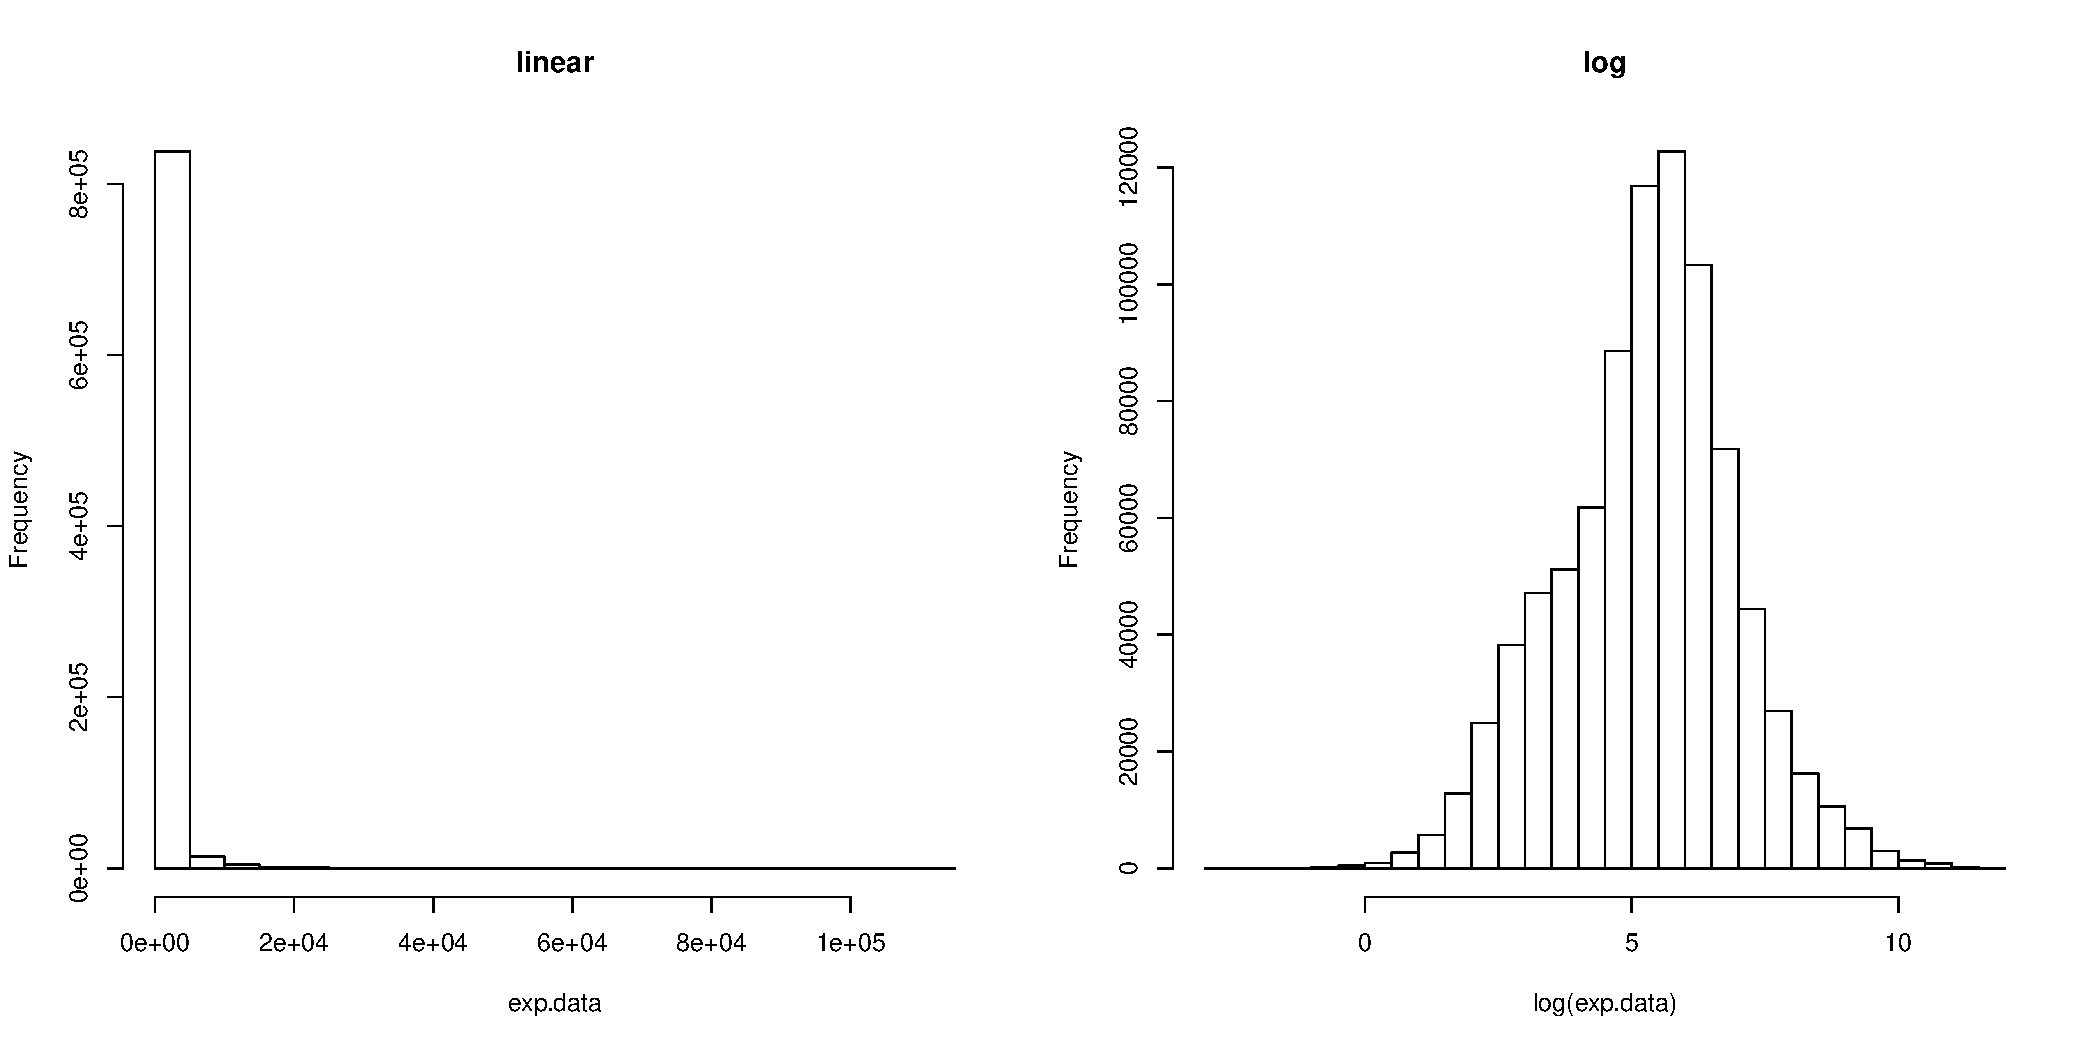
\includegraphics[width=0.8\textwidth]{images/all_hist.pdf}
  \caption{The distributions of all expression values. Left linear, and
    right log transformed values}
  \label{allhist}
\end{figure}

The distributions we obtain here are fairly typical for what global
expression values. That is that we have something that approximates
normality after log transformation. What the distribution should
actually look like is somewhat controversial (or at least it was
last time I read about it a few years ago): in any case it will depend
on the sensitivity of the measurement being used. With next generation
sequencing it is possible to increase the sensitivity by increasing
the number of sequences determined. When this is done for pure populations
of cells (a homogeneous sample) it has been reported that a bimodal
log normal distribution is observed. In fact if you look carefully at
the distribution in the right hand side it looks a little bit like it
is the sum of two distinct populations, but the sensitivity of the
array used isn't really good enough to separate the distributions
(and also remember that here we are looking at values from three
distinct tissue types).

Next we should have a look at the distributions of the individual
samples. We can use the heatmap function to look at the individual
distributions. However, first we have to understand what the
hist command does. When you call:

\begin{rcode}
  hist(log(exp.data))
\end{rcode}

the distribution for the data is determined and plotted. In addition
the \texttt{hist()} function returns an object of the class "histogram".
However, it does this invisibly. ?? This means that if you don't assign
the object returned to some variable, then it is simply discarded,
and all you get is the plot. That is often ok, but if you wish to 
compare the distributions from different populations then you will
need to store the objects and extract the relevant values.

An object of the \texttt{histogram} class, like so many other classes
in R, is simply a named list (you've seen this above for the GEOquery
function) where you can access the individual elements using the \texttt{\$}
operator. To find out what the object contains, have a look at the 
manual page for \texttt{hist} and scroll down to the "Value" section.

\begin{verbatim}
...
     breakpoints as a function of ‘x’.

Value:

     an object of class ‘"histogram"’ which is a list with components:

  breaks: the n+1 cell boundaries (= ‘breaks’ if that was a vector).
          These are the nominal breaks, not with the boundary fuzz.

  counts: n integers; for each cell, the number of ‘x[]’ inside.

 density: values f^(x[i]), as estimated density values. If
          ‘all(diff(breaks) == 1)’, they are the relative frequencies
          ‘counts/n’ and in general satisfy sum[i; f^(x[i])
          (b[i+1]-b[i])] = 1, where b[i] = ‘breaks[i]’.

    mids: the n cell midpoints.

   xname: a character string with the actual ‘x’ argument name.

equidist: logical, indicating if the distances between ‘breaks’ are all
          the same.
     Prior to R 3.0.0 there was a component ‘intensities’, the same as
     ‘density’, for long-term back compatibility.
\end{verbatim}

Hopefully this is fairly self-explanatory. If not, I can try to explain how
to read this in the session (ok, maybe the description of density may not
be particularly clear, but...). When we plot the distribution we plot the
\texttt{\$mids} component on the x-axis and then either the actual counts
(the number of values within the range) or the density (the proportion of
values within the range) on the y-axis. If we wish to compare two distributions
in the same plot we normally use the \texttt{\$density} component as
this is not affected by the total number of values. We also would like to
make sure that we use the same ranges for all the different distributions. The
specific ranges are determined by the value of the \texttt{breaks} option
passed to the \texttt{hist()} function (this is an optional parameter) and
which can be accessed from \texttt{histogram} objects in the \texttt{\$breaks}
component.

To determine a set of breakpoints which will be suitable for all the
columns of the data, we can simply let the \texttt{hist()} function
determine something that is suitable for the full data set (as we
did above). When we ran the \texttt{hist(log(exp.data))} above, we
assigned the returned value to the \texttt{h.all} object. So, we can
simply use the \texttt{breaks} component of \texttt{h.all} 
(\texttt{h.all\$breaks}) when we call hist for the individual components.

In R, if we wish to call a function on all columns or all rows of a
matrix we usually use the \texttt{apply} function. You can also loop
through the columns or rows and call the function explicitly, but
this is not considered as elegant (though that's often arguable, and
using \texttt{apply()} takes exactly the same amount of time).

The first argument of the apply function is the the data that you wish
to use, the second argument determines whether you wish to call the
function on the rows or columns of the data (1=rows, 2=columns), and
the third argument is a function to call. The last argument can
be a function definition that takes a single argument, or the name of
a function (it is also possible to supply options to the function in
additional arguments):

\begin{rcode}
  h.sample <- apply( log(exp.data), 2, function(x){ hist(x, breaks=h.all$breaks)} )
  ## here I specify the breaks option to be the same as in the histogram
  ## we obtained for the full data set (h.all$breaks)
\end{rcode}

Here the \texttt{apply} function will return a list of \texttt{histogram} objects,
one for each column. To extract the \texttt{counts} component from
each of these into a matrix that we can give to the heatmap function we can do:

\begin{rcode}
  ## the sapply function is similar to the apply function, but works
  ## with vectors and lists, and tries to simplify the output to
  ## give a matrix if possible (if all the returned vectors have the
  ## same length

  h.sample.c <- sapply(h.sample, function(x){ x$counts }
  ## remember that the last statement of a function is just returned
  ## so here the function will simply return the x$counts component
  ## which is a numeric vector
  
  ## the heatmap function likes to have row and column names,
  rownames(h.sample.c) <- h.all$mids
  ## h.all$mids are the mid point values for the ranges of the histogram
\end{rcode}

And finally to make a picture of this, we do:

\begin{rcode}
  heatmap(h.sample.c, Rowv=NA, Colv=NA, scale='none', col=rainbow(255, s=1, v=0.8))
\end{rcode}

We can make a pdf and add a bit of information to the plot by:

\begin{rcode}
  ## with column colours. But this is troublesome
  colColor <- rep('grey', ncol(h.sample.c))
  colColor[ samples[,'tissue'] == 'skeletal muscle (gastrocnemius)' ] <- 'red'
  colColor[ samples[,'tissue'] == 'liver' ] <- 'blue'
  colColor[ samples[,'tissue'] == 'adipose tissue (epididymal)' ] <- 'green'
  
  pdf("distributionHeatMap.pdf", width=10, height=10)
  heatmap(h.sample.c, Rowv=NA, Colv=NA, scale='none', col=rainbow(255, s=1, v=0.8),
  ColSideColors=colColor )
  dev.off()
\end{rcode}

\begin{figure}[ht]
  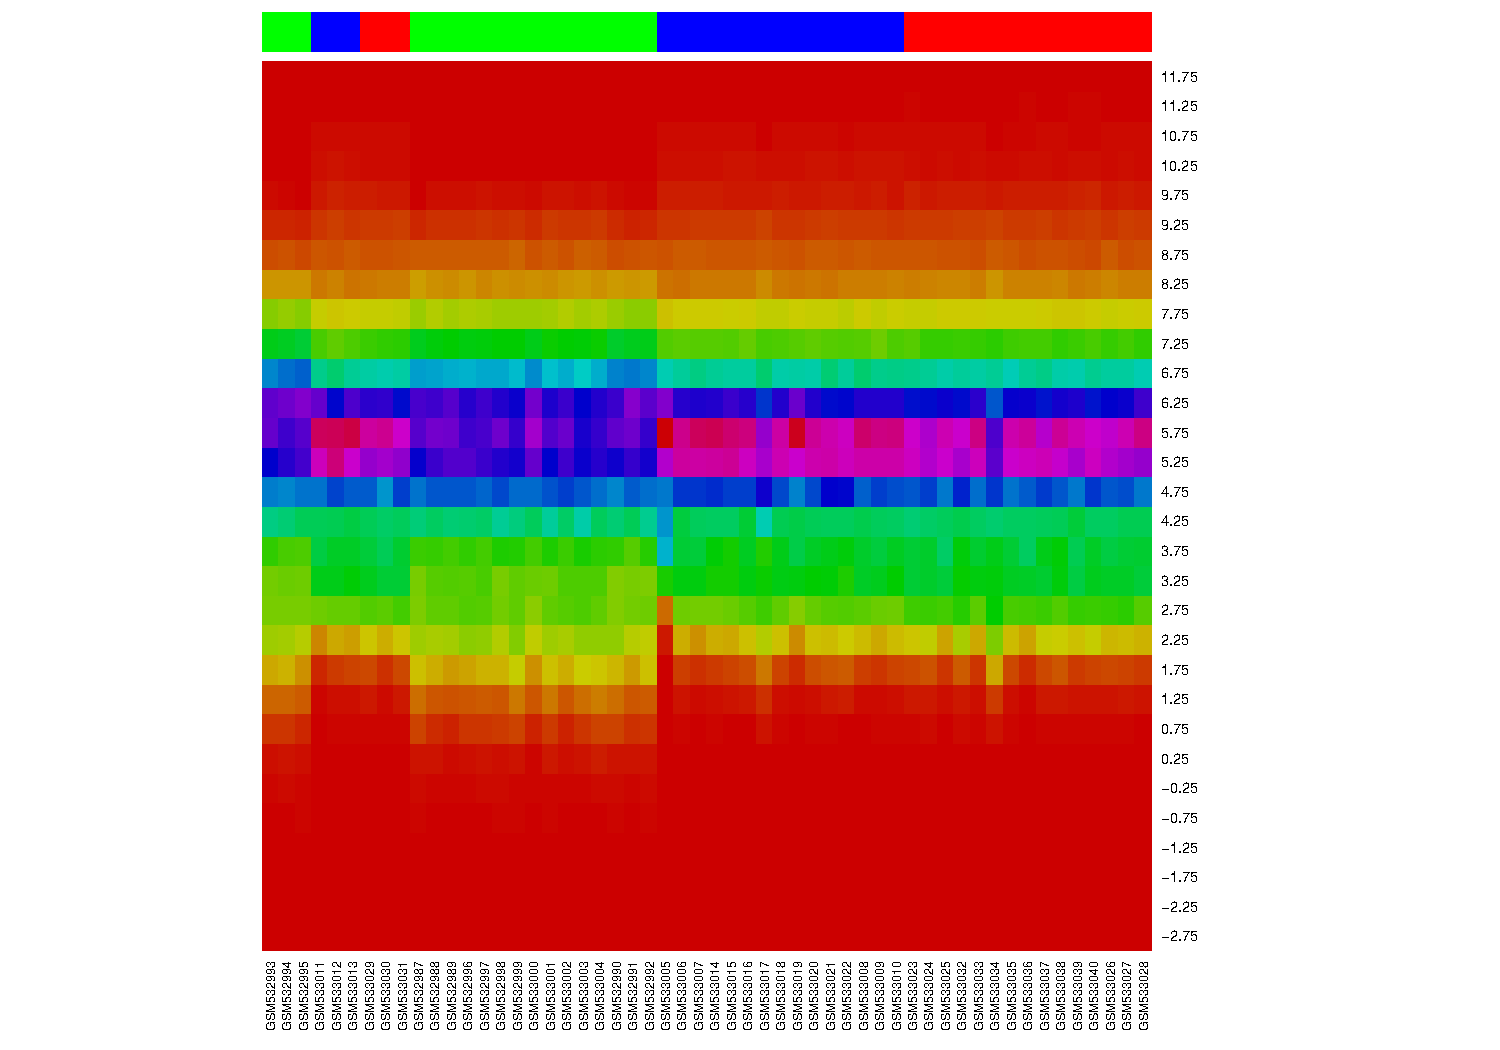
\includegraphics[width=0.6\textwidth]{images/distributionHeatMap.pdf}
  \caption{Sample log distributions plotted as a heatmap. The colors in the bar
  above the plot indicate the tissue type.}
  \label{disthm}
\end{figure}

This gives us Fig. \ref{disthm}. In general most of the distributions look
ok, but we can see that there is something different about the samples
represented by the green colour (adipose tissues). This difference in distribution
may be related to the biological nature of the samples, but it may also be
an experimental artefact. At this point it would be useful to be able to
go back to lower level data (eg. individual probe data) which might tell us
something about the cause of the discrepancy. However, that is a little advanced
for course.

We can get a rough idea of the overall distributions in a rather simpler
way by creating a boxplot for the data:

\begin{rcode}
  boxplot(log(exp.data), las=2, cex.axis=0.8)
  ## the las option makes the labels on the x-axis vertical
  ## the cex.axis option changes the size of the font of these
  ## so that the whole label can be seen. (cex = character
  ## expansion vector)
\end{rcode}

To make a pdf and add some colour to the plot we can do:

\begin{rcode}
  pdf("boxplot.pdf", width=10, height=7)
  boxplot(log(exp.data), las=2, cex.axis=0.8, col=(1+as.numeric(as.factor(samples[,'tissue']))))
  dev.off()
  ## see if you understand the col= option...
\end{rcode}

\begin{figure}[ht]
  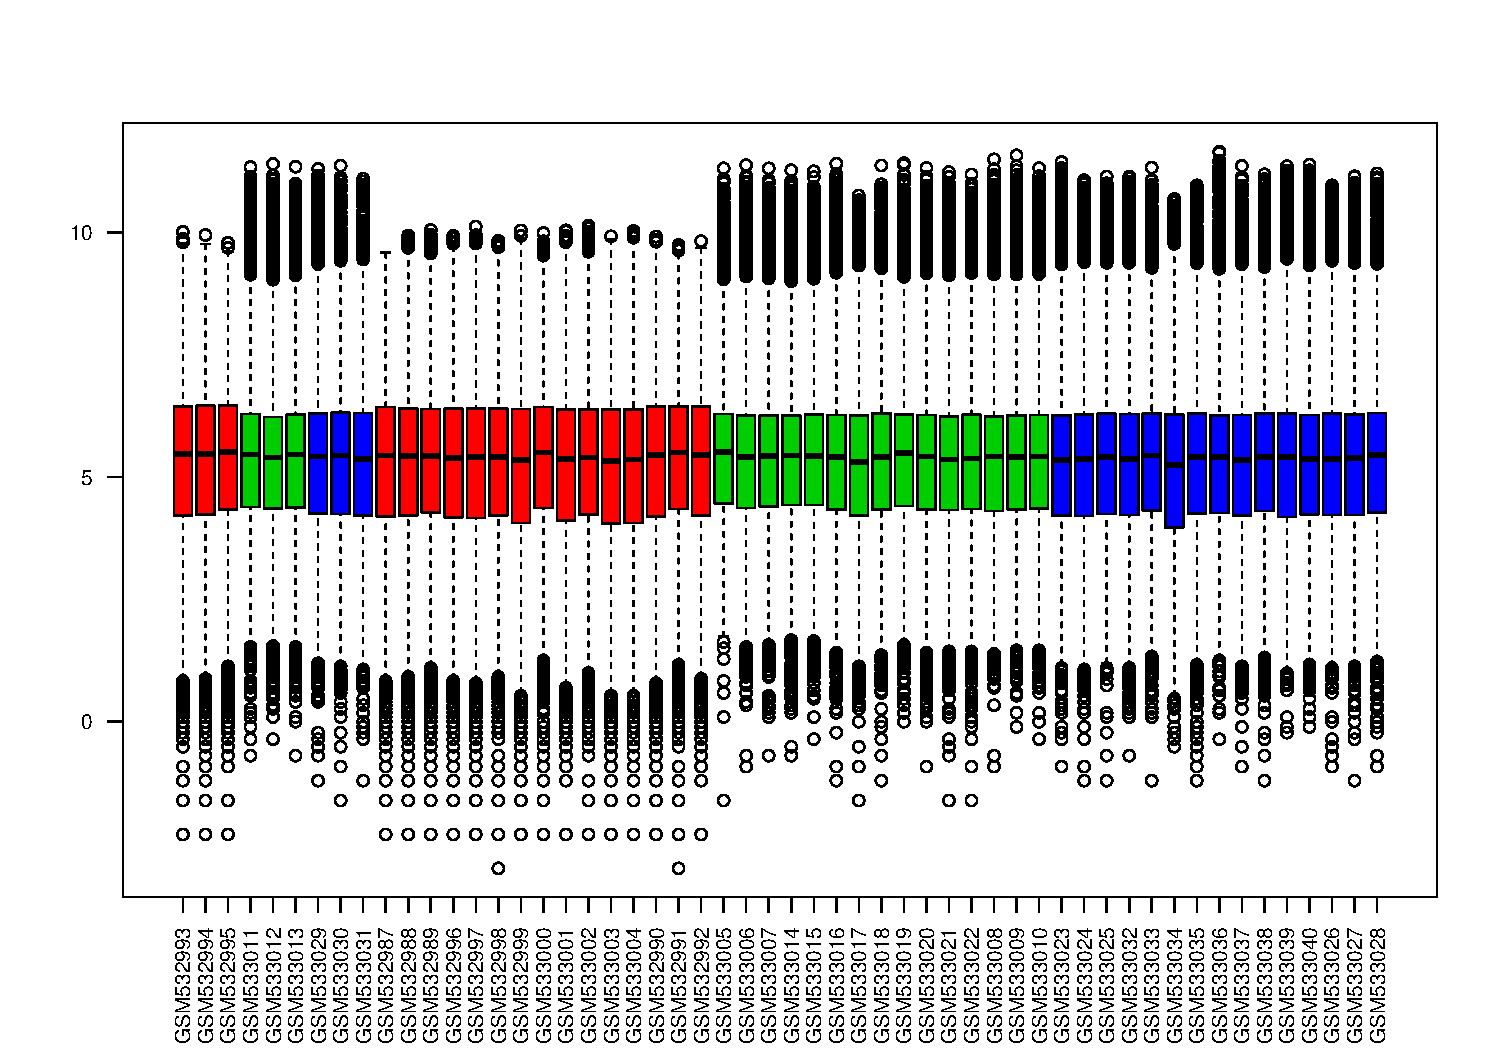
\includegraphics[width=\textwidth]{images/boxplot}
  \caption{The distributions summarised as a boxplot}
  \label{boxplot}
\end{figure}

The boxplots (Fig. \ref{boxplot}) also indicate that there is something
a little different about the adipose tissues, but providing different
details (eg. it is easy to see that the adipose tissues have lower maximal
values from the boxplot, but the full distributions tell us more about the
flattening of the distribution).

\subsubsection{Pairwise comparisons}
\label{sec-1-3-2}
When microarrays first became popular it was very common to
do pairwise comparisons between samples. This can be quite useful
to give a visualisation of how similar a pair of samples are, but
given that for a data set with $n$ samples you can do $n^2$ such
plots it's not something that I spend a lot of time doing. However
it's good to know how to do. In R, ofcourse, that is very simple.

\begin{rcode}
  ## to plot sample 1 vs 2 and 1 vs 4
  ## in a single pdf 
  pdf("pairwise1.pdf", width=14, height=7)
  par(mfrow=c(1,2))
  plot(log2(exp.data[,1]), log2(exp.data[,2]), cex=0.2, col=rgb(0,0,0,0.5))
  ## we can add a couple of lines to this
  abline(0,1, col='red')
  abline(1,1, col='red', lty=2)
  abline(-1,1, col='red', lty=2)

  plot(log2(exp.data[,1]), log2(exp.data[,4]), cex=0.2, col=rgb(0,0,0,0.5))
  abline(0,1, col='red')
  abline(1,1, col='red', lty=2)
  abline(-1,1, col='red', lty=2)
  dev.off()
\end{rcode}

Here we use log2 rather than log, since differences of 1 will correspond to
2-fold changes which makes it easier to get an idea of the changes
observed in the plot. In addition we add a couple of lines to each plot
which represent equal values and 2 fold up or down differences in expression
levels between the two samples.

\begin{figure}[ht]
  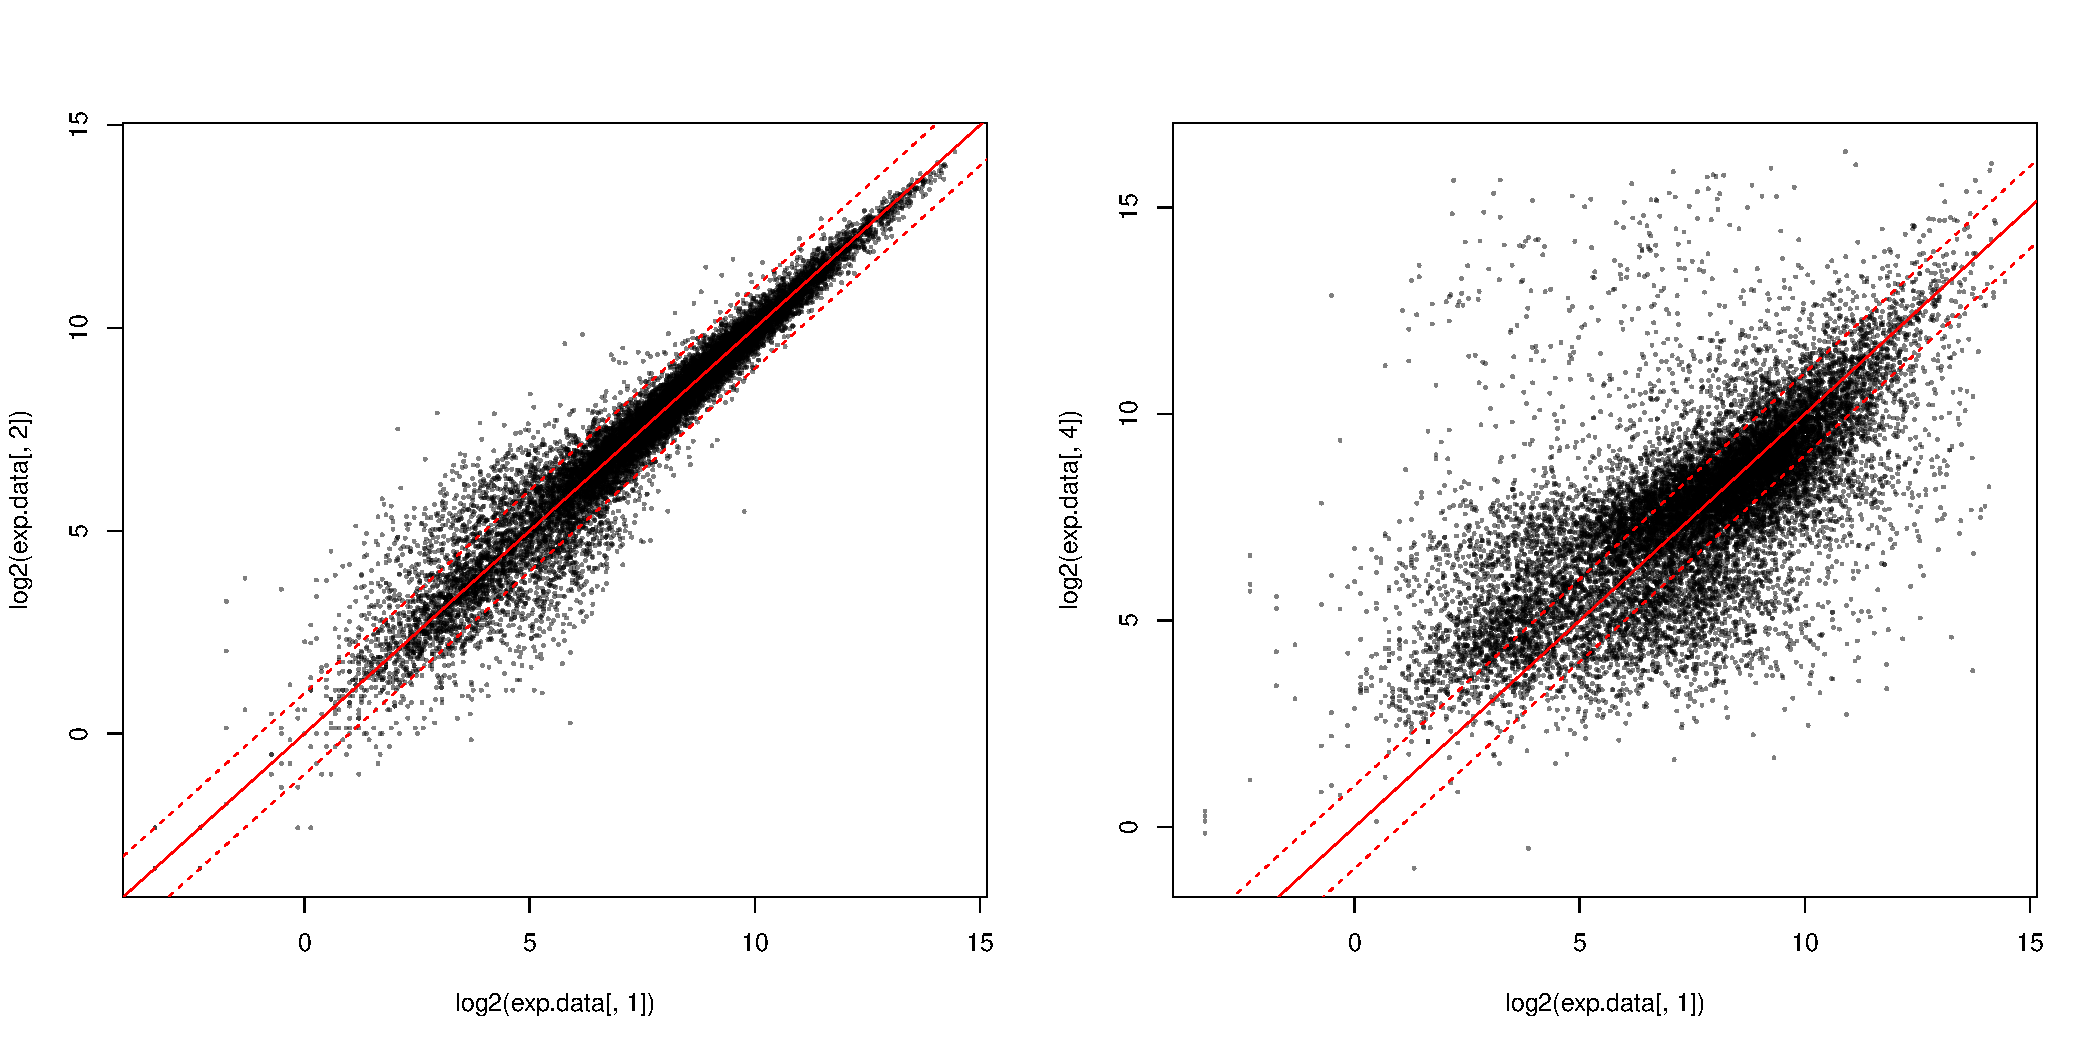
\includegraphics[width=\textwidth]{images/pairwise1}
  \caption{Pairwise plots of replicate samples (left) or samples
    from two different tissues (right)}
  \label{pairwise}
\end{figure}

From the pairwise plots (Fig. \ref{pairwise}) we can see that expression levels
in the same tissues are generally similar to each other. Not 
unexpectedly we see more differences when we compare levels between samples.
The plot between two different tissues (right panel) also suggests that we
might wish to perform additional normalisation of the data. In general, we
would expect that most of the points should lie along the diagonal, but here we
see a sort of L-shape in the plot. That is a result of the difference in the
distributions that we observed in the earlier analyses. However, we should
always be careful to normalise away such differences as they may reflect
biological differences in the samples (and here we will not do any more such
analysis).

\subsubsection{An overview of the samples using PCA}
\label{sec-1-3-2}
Each sample in the data set is described by its set of expression levels; in this way we
can consider that each sample occupies a position in N-dimensional space (where N is
around 15,000, so rather large). We can easily calculate distances between points in
N-dimensional space (these are similar to correlations between the sample vectors). It
is clear that rotating the data points in space has no effect on these sample to
sample distances, and also that the full set of inter-sample distances can be represented
in $(n-1)$ dimensional space (where $n$ is the number of samples). This can most easily
be understood by imagining three points in N-dimensional space; the three points form
a plane and if that plane is rotated such that it lies in the first two dimensions
we can visualise the relationships between the samples in 2 dimensions. Similarly,
for 4 points in $N$ dimensions these will form a tetrahedron which can be represented
fully in 3 dimensional space.

A PCA (Principal Components Analysis) performs a rotation such as to maximise the
amount of variance within the the lower dimensions. This allows the structure of
the data to be visualised. Generally only the lower two or three dimensions of a
PCA are used, but this very much depends on the nature of the data. Crucially a PCA
relies on the presence of correlation in the patterns between features, and in
the absence of such correlation the PCA will not be useful for visualising sample
relationships (but the analysis will nevertheless tell you this). Understanding
what a PCA does, and how it does it, is not particularly simple; so we will just
do it, and hopefully some feeling of what the analysis does will stick in your mind.

\begin{rcode}
  ## use the prcomp functin after transposing the data
  ## (otherwise we'll rotate points representing the features
  ## not the samples. This can also be interesting, but for now
  ## keep it simple.
  pca.l1 <- prcomp(t(log(exp.data)), scale=TRUE)
\end{rcode}

Setting the \texttt{scale} option to \texttt{TRUE} means that the pattern
of expression for each gene will be scaled across the experimental series.
If we don't do this, genes with higher expression values will have a larger
impact on the result than genes with low levels of expression. Whether this is
appropriate depends on the biological question, but in gengeral when dealing
with gene expression it is better to scale the data.

If we simply call plot on the returned object it will give a plot of the
variances associated with each dimension. In this case we can see that
almost all of the variance is in the first two dimensions of the 
rotated data.

The \texttt{prcomp} function returns a named list which is described (as
usual) in the \texttt{Value} section of the documentation:

\begin{verbatim}
     constant (for ‘center = TRUE’) variables.

Value:

     ‘prcomp’ returns a list with class ‘"prcomp"’ containing the
     following components:

    sdev: the standard deviations of the principal components (i.e.,
          the square roots of the eigenvalues of the
          covariance/correlation matrix, though the calculation is
          actually done with the singular values of the data matrix).

rotation: the matrix of variable loadings (i.e., a matrix whose columns
          contain the eigenvectors).  The function ‘princomp’ returns
          this in the element ‘loadings’.

       x: if ‘retx’ is true the value of the rotated data (the centred
          (and scaled if requested) data multiplied by the ‘rotation’
          matrix) is returned.  Hence, ‘cov(x)’ is the diagonal matrix
          ‘diag(sdev^2)’.  For the formula method, ‘napredict()’ is
          applied to handle the treatment of values omitted by the
          ‘na.action’.

center, scale: the centering and scaling used, or ‘FALSE’.
\end{verbatim}

Normally we are most intersted in the \texttt{x} component. To plot the PCA
we can do:

\begin{rcode}
 pdf("pca_variances.pdf", width=7, height=7)
 plot(pca.l1)
 dev.off()

 pdf("pca_dim_1_2.pdf", width=7, height=7)
 plot(pca.l1$x[,1], pca.l1$x[,2], col=as.factor(samples[,'tissue']),
      pch=19)
 ctl.b <- samples[,'drug'] == 'control'
 points(pca.l1$x[ctl.b,1], pca.l1$x[ctl.b,2], col='purple', 
      lwd=2, pch=1, cex=2)
 dev.off()
\end{rcode}

This will give us a plot of the variances (Fig. \ref{pcaVar}) and a plot
of the first two dimensions of the rotated data (Fig. \ref{pca12}) where
we have used colour to indicate the tissue type and have highlighted
the control samples (i.e. no drug) using circles around the points.

\begin{figure}[ht]
  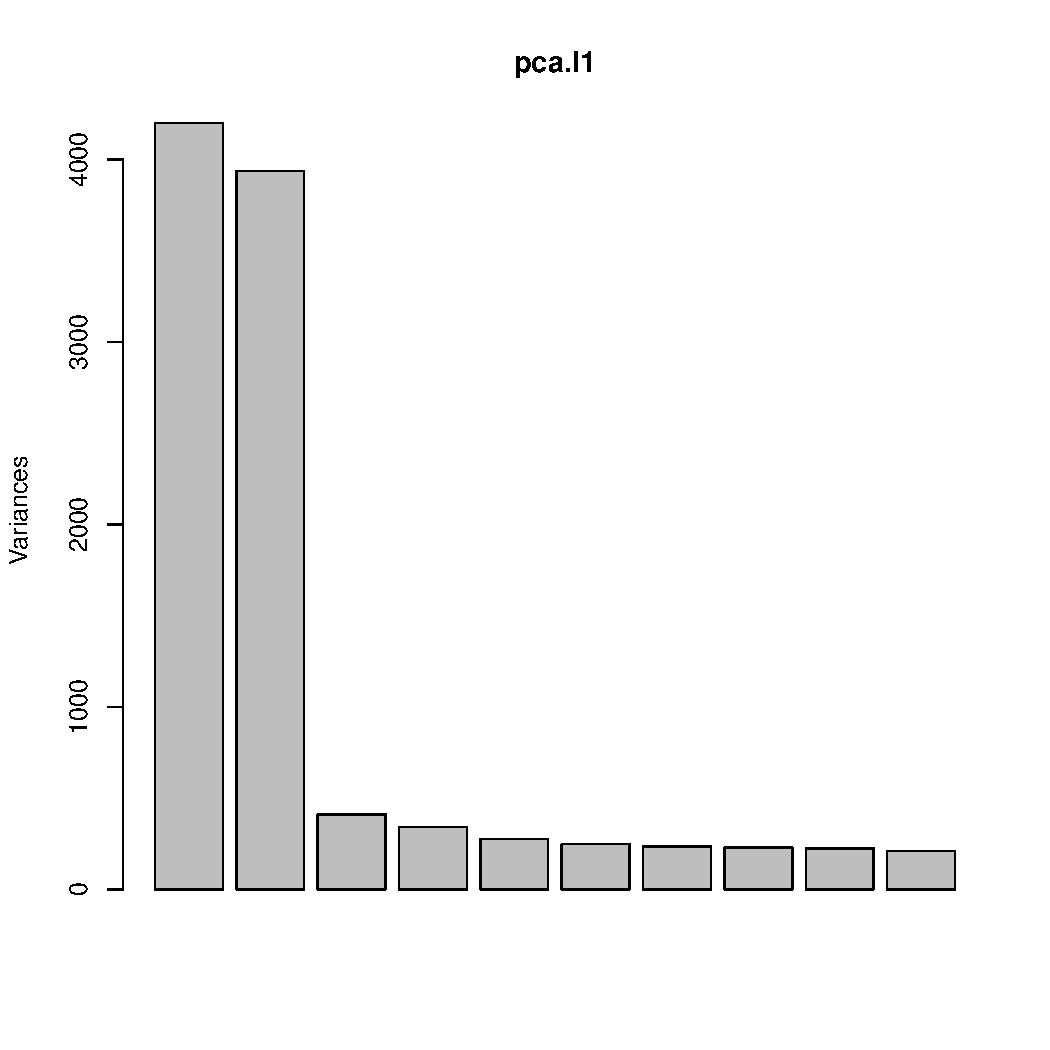
\includegraphics[width=0.7\textwidth]{images/pca_variances.pdf}
  \caption{The variances of the PCA dimensions}
  \label{pcaVar}
\end{figure}

\begin{figure}[ht]
  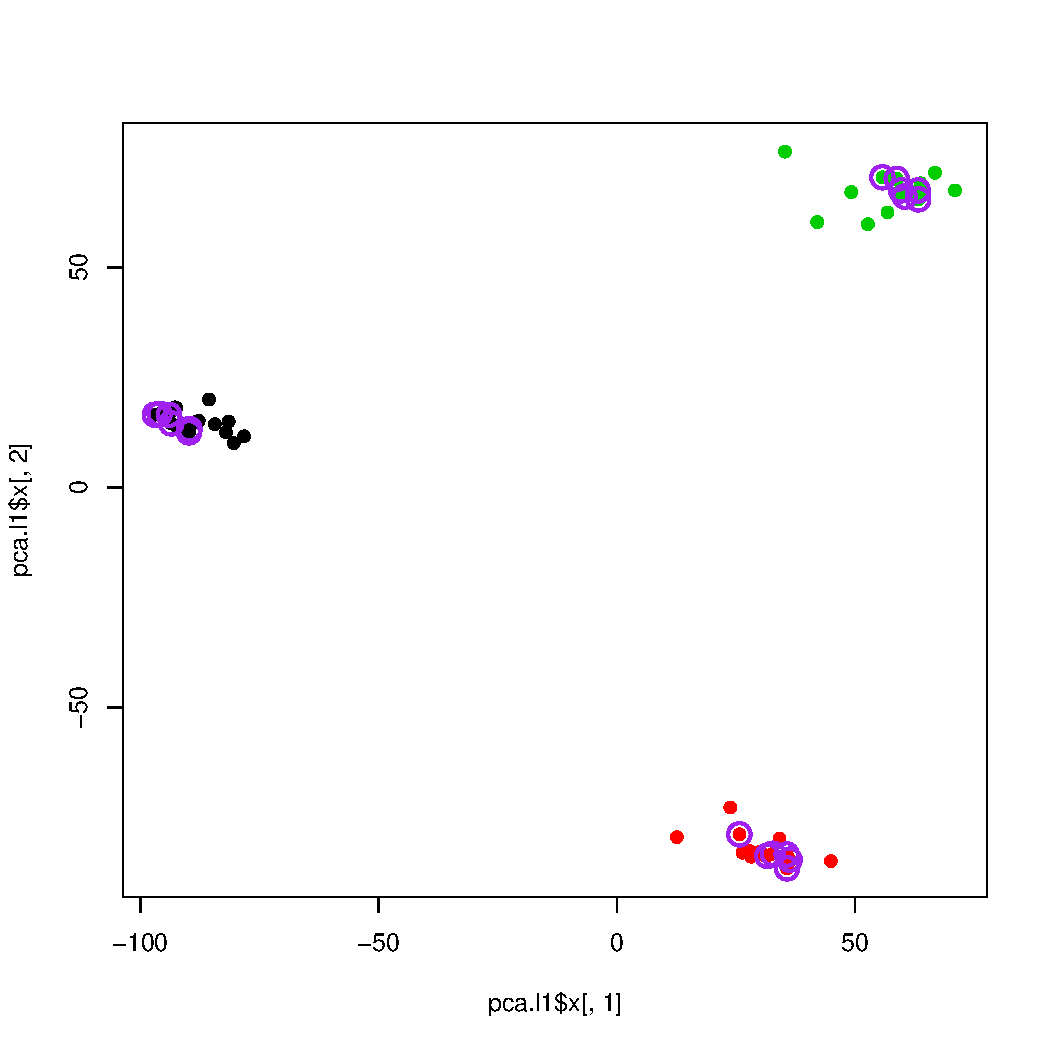
\includegraphics[width=0.7\textwidth]{images/pca_dim_1_2.pdf}
  \caption{The first two dimensions of the PCA. Colours indicate tissue type,
    circles indicate control samples with no drug treatment}
  \label{pca12}
\end{figure}

You can also look at how similar the different samples are using the correlations
between samples. Given a single matrix, the \texttt{cor} function will calculate
the correlations between columns (see \texttt{?cor}, for how this is done; there
are several options). This will give a matrix that can be plotted using the
heatmap function as above.

\begin{rcode}
  sample.cor <- cor(log(exp.data))
  pdf("sample_correlation.pdf", width=10, height=10)
  heatmap(sample.cor, scale='none', col=rainbow(255, v=0.8))
  dev.off()
\end{rcode}

\begin{figure}[ht]
  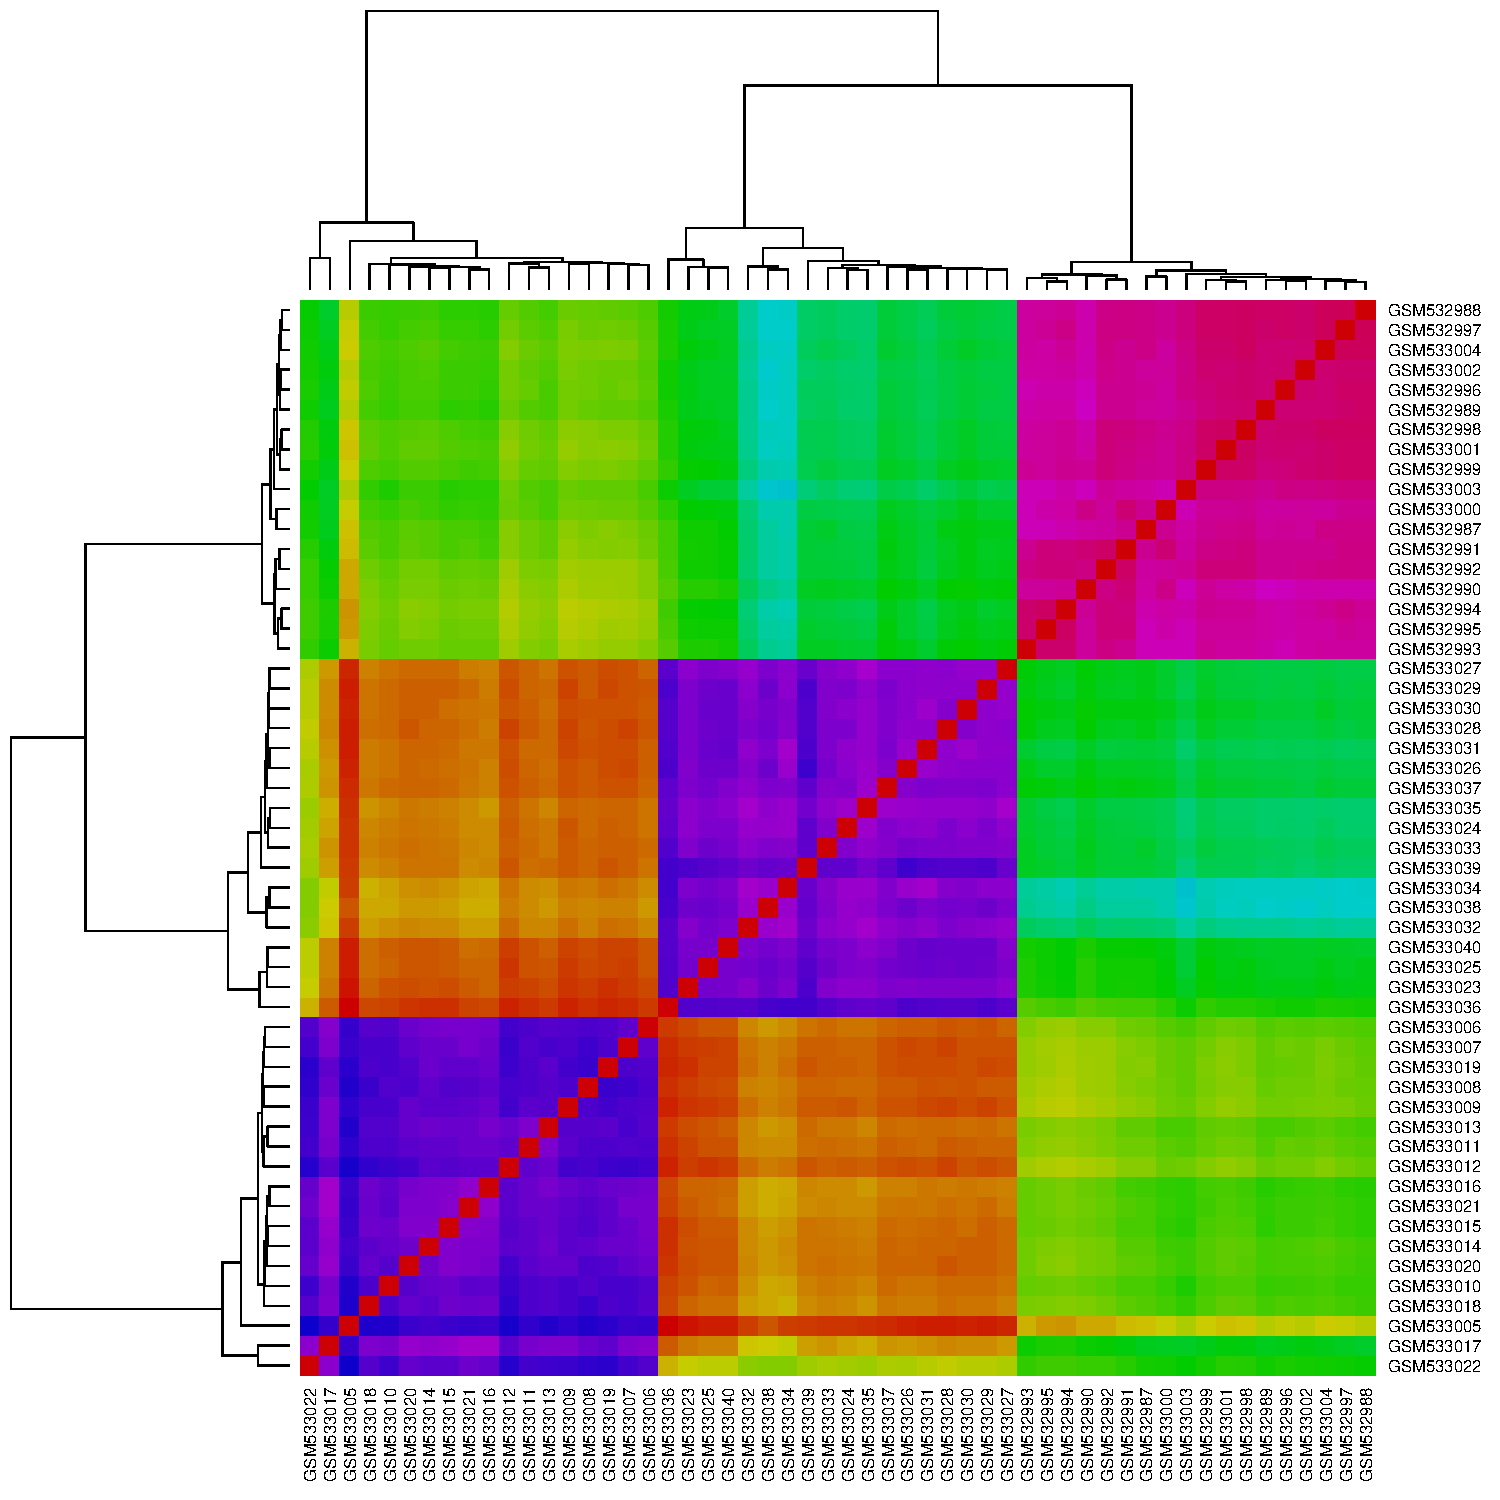
\includegraphics[width=\textwidth]{images/sample_correlation}
  \caption{Intersample correlations also indicate the tissue type}
  \label{corplot}
\end{figure}

The plot of intersample correlations (Fig. \ref{corplot}) also indicates
the very strong effect that tissue type has on the expression levels. It
also gives some indication as to which tissue types are more similar to each
other. In this case I've allowed the heatmap to cluster the samples along
the axis to group similar samples close to each other. Heatmap makes
use of the \texttt{hclust} function which builds a tree based on the 
correlations between the samples. This is very similar to the kind of trees
that we discuseed in the multiple alignment lecture.

\newpage


\subsubsection{Identifying some interesting features}
\label{sec-1-3-3}
To identify some interesting features we will calculate f-statistics for
individual transcripts. We can calculate such statistics either for
the full data set and all the experimental factors or we can make
use of subsets of the data and factors. Here we will calculate for
the full set of groupings and for drug effect within the liver samples.
We will then plot some of transcripts to see a few different ways in
which we can visualise patterns.

To get fstatistics we will use a couple of functions in the
\texttt{general\_functions.R} file, which I have made available on
fronter today. We will also use the \texttt{mulFactor} function that
gives us a way to define sample factors in a convenient manner.


\begin{rcode}
## first make sure to copy the general_functions.R file
## into the directory that you are using for R
source("general_functions.R")

## get a set of factors
sample.mf <- mulFactor(samples, c('genotype', 'tissue', 'drug'))
## look at what you got, and see if it makes sense to you
sample.mf$f
sample.mf$m

## use fStats to get some statistics for everything
fstats.a <- fStats(log(exp.data), sample.mf$f)

## then lets get the stats for just the liver samples and 
## drug treatment
liver.b <- samples[,'tissue'] == 'liver'
fstats.dl <- fStats(log(exp.data[,liver.b]), as.numeric(as.factor(samples[liver.b,'drug'])))

## this gives us the order of the liver drug influence fstats
fstats.dl.o <- order(fstats.dl$f, decreasing=TRUE)

## plot the levels, using the plotExp function (see below)
## note that you have to define the plotExp function before you can do this

plotExp( fstats.dl.o[1:10] )

## get an order for the full fstats and have a look yourselves!
\end{rcode}

The plotting function:

\begin{rcode}
## this function makes use of global variables. These can't be modified,
## but can still result in unexpected behaviour
plotExp <- function(ind, interactive=TRUE){
  for(j in ind){
    #j <- ind[i]
    mx <- max(exp.data[j,])
    mn <- min(exp.data[j,])
    plot(1:length(sample.o), exp.data[j, sample.o],
    type='n', col=as.factor(samples[sample.o,'drug']), pch=19,
    ylim=c( mn - (mx-mn)*0.05, mx ),
    main=paste(feat.data[j,'Gene symbol']), ylab='Expression', xlab='Sample')
    usr <- par("usr")
    ## set up some rectangles to indicate the tissue type.
    rect((1:length(sample.o))-0.5, usr[3], (1:length(sample.o))+0.5, usr[4],
    col=hsvScale(as.numeric(as.factor(samples[sample.o,'tissue'])), sat=0.5, alpha=0.5),
    border=NA)
    ## and to indicate the genotype
    rect((1:length(sample.o))-0.5, usr[3], (1:length(sample.o))+0.5, usr[3] + (mx-mn)*0.05,
    col=hsvScale(as.numeric(as.factor(samples[sample.o,'genotype'])), sat=c(0.5), alpha=0.6),
    border=NA)
    
    points(1:length(sample.o), exp.data[j, sample.o], type='b',
    pch=19, col=as.factor(samples[sample.o,'drug']) )
    if(interactive)
    inp <- readline(paste(feat.data[j,'Gene symbol'], ":"))
  }
}
\end{rcode}

You can find this at the end of the "exp\_analysis.R" file which I will also 
make available on fronter.

Good luck!

\end{document}
